\section{Bridging Gadgets}

\begin{frame}{Recall: Many width-3 gadgets.}

\begin{columns}[T,totalwidth=\linewidth]

\column{0.49\linewidth}
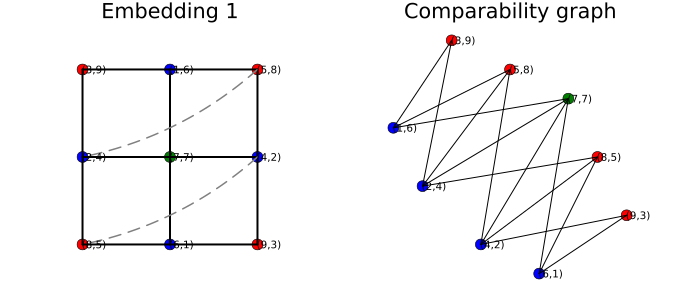
\includegraphics[width=\linewidth]{media/collage/img1}

\vspace{0.02\linewidth}

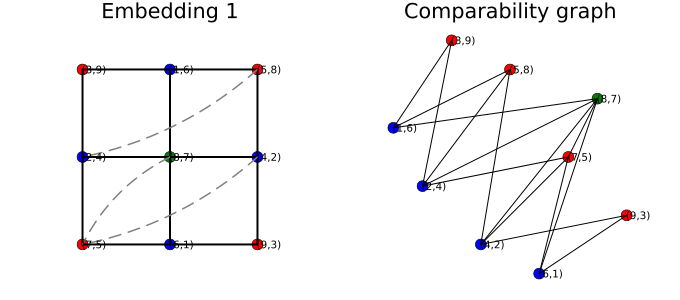
\includegraphics[width=\linewidth]{media/collage/img3}

\vspace{0.02\linewidth}

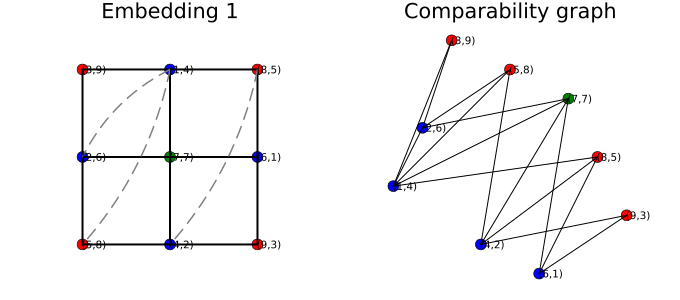
\includegraphics[width=\linewidth]{media/collage/img5}

\column{0.49\linewidth}
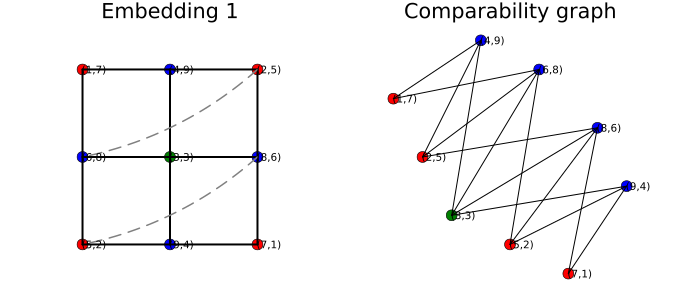
\includegraphics[width=\linewidth]{media/collage/img2}

\vspace{0.02\linewidth}

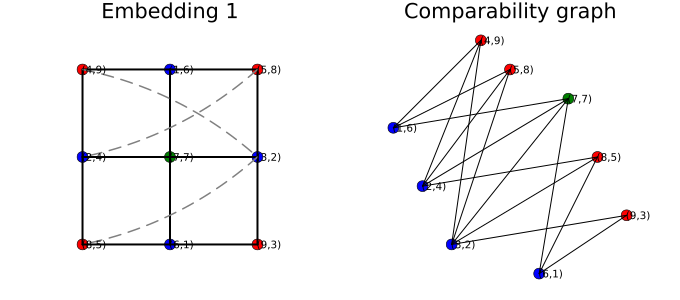
\includegraphics[width=\linewidth]{media/collage/img4}

\vspace{0.02\linewidth}

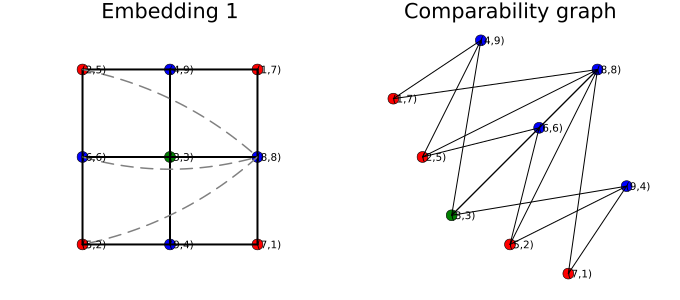
\includegraphics[width=\linewidth]{media/collage/img6}

\end{columns}

\end{frame}

\begin{frame}{Bridging Gadgets: Informal Visual Definition}

\begin{columns}[T,totalwidth=\linewidth]

\column{0.4\linewidth}

\begin{center}  
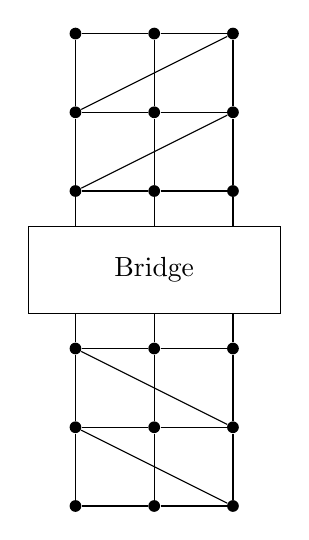
\begin{tikzpicture}[scale=1,
    dot/.style={circle, fill, inner sep=1.5pt},
    bridge/.style={draw, rectangle, minimum width=3.2cm, minimum height=1.1cm}
]

% Top 3x3 grid vertices
\foreach \x in {0,1,2}{
    \foreach \y in {0,1,2}{
        \node[dot] (T\x\y) at (\x, 4+\y) {};
    }
}

% Top grid edges
\foreach \x in {0,1,2}{
    \foreach \y in {0,1}{
        \draw (T\x\y) -- (T\x\the\numexpr\y+1\relax);
        \draw (T\y\x) -- (T\the\numexpr\y+1\relax\x);
    }
}

\draw (T00) -- (T21);
\draw (T01) -- (T22);

% Bottom 3x3 grid vertices
\foreach \x in {0,1,2}{
    \foreach \y in {0,1,2}{
        \node[dot] (B\x\y) at (\x, \y) {};
    }
}

% Bottom grid edges
\foreach \x in {0,1,2}{
    \foreach \y in {0,1}{
        \draw (B\x\y) -- (B\x\the\numexpr\y+1\relax);
        \draw (B\y\x) -- (B\the\numexpr\y+1\relax\x);
    }
}

\draw (B02) -- (B21);
\draw (B01) -- (B20);

% Bridge ellipse centered between grids
\node[bridge] (bridge) at (1,3) {Bridge};

% Define 3 attachment points on top and bottom of bridge, aligned with x=0,1,2
\foreach \x in {0,1,2}{
  \coordinate (bn\x) at (\x, 3+0.55); % near top of ellipse
  \coordinate (bs\x) at (\x, 3-0.55); % near bottom of ellipse
}

% Vertical edges from bottom row of top grid (y=4) down into bridge
\foreach \x in {0,1,2}{
  \draw (T\x0) -- (bn\x);
}

% Vertical edges from top row of bottom grid (y=2) up into bridge
\foreach \x in {0,1,2}{
  \draw (B\x2) -- (bs\x);
}

\end{tikzpicture}

\end{center}

\column{0.6\linewidth}

\begin{definition}[Informal]
A width-3 bridge of size $b \in \mathbb{N} \cup \{0\}$ adds $3b$ new vertices between two width-3 gadgets. The bridge has some $\Grid_{3 \times b}$ as a subgrid.
\end{definition}

\vspace{0.5cm}

\only<2->{
The bridge can have any number of additional edges; set $\theta = 0$ to ``ignore'' them.
}

\vspace{0.5cm}

\only<3->{
Question: Given width-3 gadgets $A$ and $B$, how can we construct a width-3 bridge of size $b$ or prove that it is impossible?
}

\end{columns}

\end{frame}

\begin{frame}{Linear Programming Bridging Algorithm}

\begin{definition}[Informal]
Given width-3 gadgets $A$ and $B$, encode each as inequalities on a linear program.
\end{definition}

\begin{example}
Suppose we are dealing with width-2 gadgets and $A$ has $\pi(A) = (2,1,4,3)$. We add conditions:
\begin{align}
    x_1 < x_2 < x_3 < x_4 \\
    y_2 < y_1 < y_4 < y_3.
\end{align}
\end{example}
\end{frame}

\begin{frame}{Linear Programming Bridging Algorithm cont'd}

\begin{lemma}[Informal]
We can add additional inequalities to a linear program encoding $A$ to also encode $B$ and any bridge vertices.
\end{lemma}

\begin{theorem}
Fix a bridge size $b$. If the corresponding linear program is infeasible, then there is no bridge of size $b$ between $A$ and $B$.
\end{theorem}

\begin{fact}<2->
There exists no bridge of size $b < 4$ between any two width-3 gadgets $A$, $B$, where each gadget has at most 3 additional edges compared to $\Grid_{3 \times 3}$.
\end{fact}

\begin{proof}<3->
Brute force every linear program encoding of ordered pairs of gadgets $A,B$ with at most 3 additional edges.
\end{proof}

\end{frame}